% graphics source https://docs.google.com/presentation/d/111HE56Ow0miZApHPBa18eyPAw8cdslZyBCavoWMix8E
\begin{figure}

\begin{minipage}{0.5\linewidth}
\centering
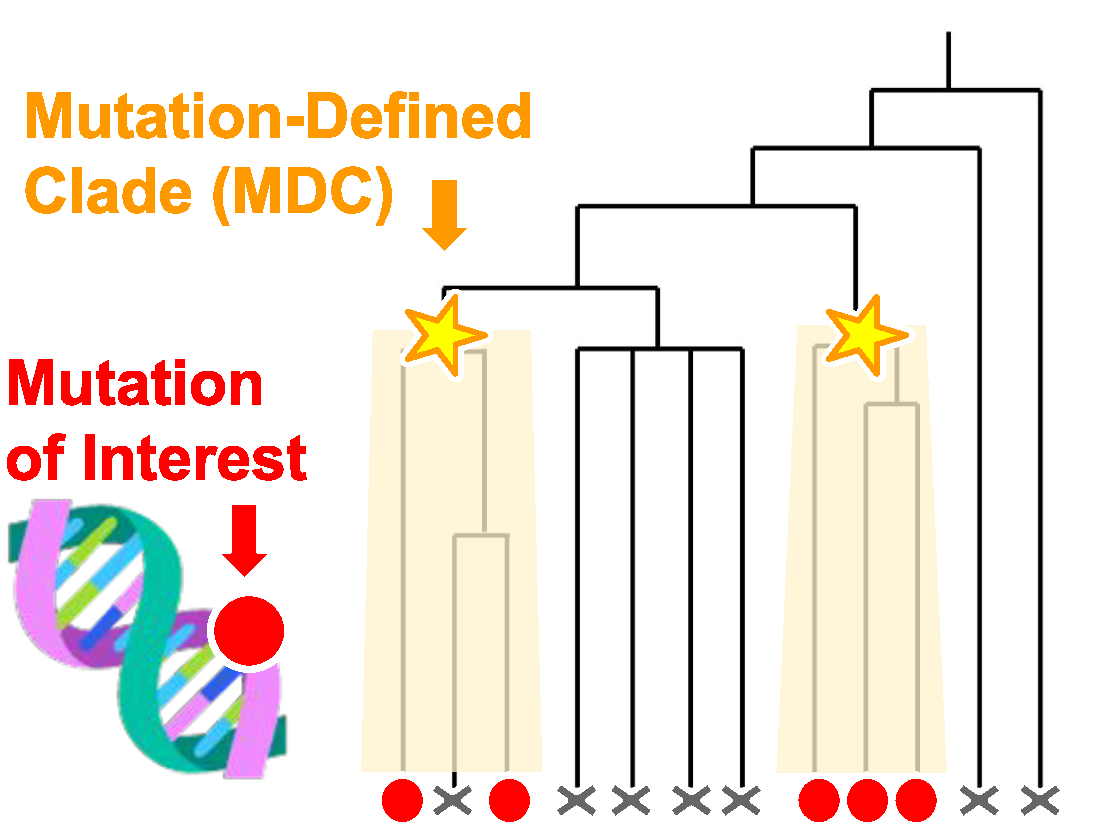
\includegraphics[width=\linewidth]{img/mls-schematic-mdc}
\subcaption{mutation-defined clades}
\label{fig:mls-schematic:mdc}
\end{minipage}%
\begin{minipage}{0.5\linewidth}
\centering
\begin{minipage}{\linewidth}
\centering
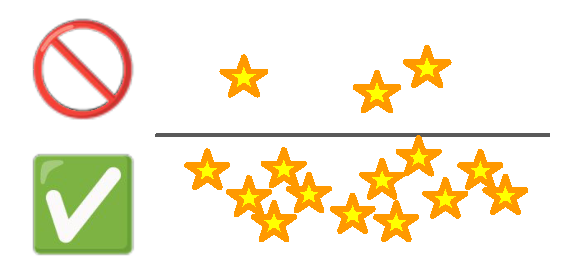
\includegraphics[width=0.8\linewidth]{img/mls-schematic-mutfreq}
\subcaption{mutation frequency}
\label{fig:mls-schematic:mutfreq}
\end{minipage}
\begin{minipage}{\linewidth}
\centering
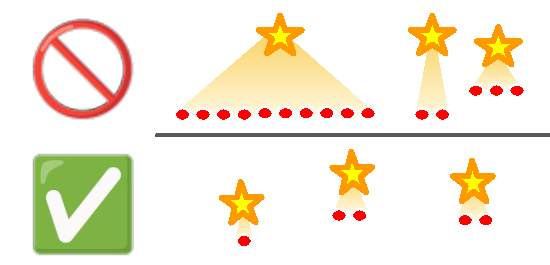
\includegraphics[width=0.8\linewidth]{img/mls-schematic-fiteffect}
\subcaption{fitness effect}
\label{fig:mls-schematic:fiteffect}
\end{minipage}
\end{minipage}

\caption{\textbf{Adapted method to screen for multilevel selection on an example mutation of interest.} a) The phylogeny for the mutation of interest. In this case, the mutation arises twice (indicated by stars), producing two mutation-defined clades (highlighted in yellow). Red circles indicate leaf taxa with the mutation. b) Mutations under MLS should be observed more often than expected by chance. c) Mutations under MLS should go on to produce smaller clades than expected by chance.}
\label{fig:mls-schematic}

\end{figure}
